\documentclass[a4paper,11pt]{article}

\usepackage[activate={true,nocompatibility}]{microtype}
\usepackage[T1]{fontenc}
\usepackage{microtype}
%\usepackage{mlmodern}
\usepackage{Baskervaldx}
\usepackage{inconsolata}
\usepackage{xcolor}
\usepackage[utf8]{inputenc}
\usepackage[english]{babel}
\usepackage[a4paper, left=1.1in, right=1.1in]{geometry}
\usepackage{calc}

\usepackage{titlesec}
\titleformat{\subsubsection}[runin]
  {\normalfont\itshape}
  {\normalfont\bfseries(\thesubsubsection)}
  {1.5\wordsep}
  {}
  [.]

\titlespacing*{\subsubsection}
  {0pt}{1.7ex}{\wordsep}  % left, before, after spacing

\usepackage{mathpartir}
\usepackage{amsmath}

\usepackage{listings}
\lstdefinestyle{wasm}{
  basicstyle=\ttfamily,
  numberstyle=\footnotesize,
  numbers=left,
  columns=fullflexible,
  numbersep=10pt,
}
\lstset{style=wasm}

\DeclareMathOperator{\reft}{\textsf{ref}}
\DeclareMathOperator{\rect}{\textsf{rec}}
\DeclareMathOperator{\parat}{\textsf{param}}
\DeclareMathOperator{\rest}{\textsf{result}}
\DeclareMathOperator{\strt}{\textsf{struct}}
\DeclareMathOperator{\arrt}{\textsf{array}}
\DeclareMathOperator{\funt}{\textsf{func}}
\DeclareMathOperator{\fldt}{\textsf{field}}
\DeclareMathOperator{\vart}{\textsf{var}}
\DeclareMathOperator{\cstt}{\textsf{const}}
\DeclareMathOperator{\broncast}{\textsf{br\_on\_cast}}
\DeclareMathOperator{\reftest}{\textsf{ref.test}}
\DeclareMathOperator{\localget}{\textsf{local.get}}
\DeclareMathOperator{\refnullt}{\textsf{ref null}}

\usepackage{tikz}
\usepackage{wrapfig}

\usepackage[backend=bibtex, style=alphabetic]{biblatex}
\addbibresource{report/report.bib}
\author{Aghilas Y. Boussaa \texttt{<aghilas.boussaa@ens.fr>}}

\title{\textsf{watib}: An optimising toolchain for modern WebAssembly}
\begin{document}
\sloppy
\maketitle
\begin{abstract}
  WebAssembly (Wasm) is a code format aiming at providing efficient execution.
  It now offers the features needed to be a compilation target for functional
  programming languages such as Scheme. Such a backend has been developed in
  the Bigloo compiler, relying on an external toolchain.

  We present \textsf{watib}, a WebAssembly Toolchain written In Bigloo. It has
  been integrated in the Bigloo Scheme compiler and is available as a standalone
  tool. We describe \textsf{watib}'s architecture and compare our toolchain with
  the one used before.
\end{abstract}

\section{Introduction}
In 2024, a Wasm backend was added to the Bigloo Scheme compiler~\cite{Bigloo}.
It generated textual Wasm and relied on an external tool for the assembly.
\textsf{Watib} has been developed as a replacement for this tool and has been
directly integrated in the Bigloo compiler. It is also available as a standalone
tool with a command-line
interface\footnote{\url{https://www.normalesup.org/~boussaa/watib/}}.

The rest of this section gives a high-level overview of WebAssembly and
\textsf{watib}. Section~\ref{val} details \textsf{watib}'s typechecker.
Section~\ref{opt} describes the design of the different optimisation passes and
the overall design of the optimiser. Section~\ref{bench} compares
\textsf{watib}'s and existing tools' performances. We omit the assembly phase
as, once we have an intermediate representation, it is a straightforward
transcription of the specification.
\subsection{WebAssembly}
WebAssembly~\cite{haas2017bringing} is an assembly-like language for a
stack-based virtual machine. It aims at providing a fast, safe and portable
language endowed with a portable and efficient representation. New compilers
targeting Wasm are developed~\cite{emscripten, kotlin, ocaml}.

\subsubsection{Syntaxes}
The WebAssembly standard~\cite{WebAssemblyCoreSpecification3} specifies typing
rules (called validation rules), opertational semantics, an abstract syntax and
two concrete syntaxes (formats) for the language. The binary format represents
WebAssembly modules as a sequence of bytes. Wasm virtual machines such as
V8~\cite{V8} or SpiderMonkey~\cite{SpiderMonkey} and manipulated by toolchains
such as binaryen~\cite{Binaryen} or wasm-tools~\cite{WasmTools} recieve this
format. The textual format represents WebAssembly modules as S-expressions.
Toolchains receive this format and humans (and compilers such as Bigloo) write
it.

\subsubsection{New features}
The third version of the standard the standard adds features facilitating
compiling from functional languages. Wasm has now a garbage collector,
instructions for tail-calls (they are needed because the language doesn't
support goto) and exceptions. This version is still in draft, but the mentioned
features are stable and already implemented by the major Wasm engines. Bigloo's
Wasm backend relies on these features.

\subsubsection{An Example}
The example of Figure~\ref{ex} demonstrates the features evoked earlier. For a
more detailed introduction to WebAssembly,
see~\cite[Section~2.1]{phipps2023continuing} or~\cite{haas2017bringing}. This
program starts by defining a type of integer lists (\texttt{\$pair-nil}) which
is a super-type of non-empty integer lists (\texttt{\$pair}). A non-empty list
has a head (field \texttt{\$car}) which is a 32-bit integer and a tail which is
a list. The function \texttt{\$has-zero} checks whether or not a given list
contains 0. It returns a \textsf{i32} as Wasm has no boolean. The emptiness of
the list is checked by checking that the argument of type \texttt{\$pair} using
the instruction \textsf{ref.test}. The head and tail of the list can then be
accessed after it has been cast to the type \texttt{\$pair} using the
instruction \textsf{ref.cast}. Otherwise, the program wouldn't be well-typed.

\begin{figure}[h]
  \begin{minipage}{\widthof{(type \$pair (sub \$pair-nil (struct (field \$cdr (ref \$pair-nil))}}
\begin{lstlisting}
(type $pair-nil (sub (struct)))
(type $pair (sub $pair-nil (struct (field $cdr (ref $pair-nil))
                                   (field $car i32))))
(func $has-zero
  (param $l (ref $pair-nil))
  (result i32)
  (if (ref.test (ref $pair) (local.get $l))
    (then
      (if (i32.eqz (struct.get $pair $car
                     (ref.cast (ref $pair) (local.get $l))))
        (then (return (i32.const 1)))
        (else
          (return_call $has-zero
            (struct.get $pair $cdr
              (ref.cast (ref $pair) (local.get $l)))))))
    (else (return (i32.const 0))))
  (unreachable))
\end{lstlisting}
  \end{minipage}

  \caption{A Wasm function testing if a list of integers contains 0}\label{ex}
\end{figure}

\subsection{Watib}
\textsf{Watib} handles type checking (the \texttt{Val} folder of the sources),
optimisation (the \texttt{Opt} folder) and assembly (the \texttt{Asm} folder) of
Wasm programs given in textual format\footnote{binary format is planned}.
Function validation and optimisation can run in parallel. We added the option to
run them in an arbitrary number of threads using the \textsf{pthreads} library.
This feature, and thus the dependency on an external library is optional which
is required for integration with the Bigloo compiler.

The WebAssembly platform is in constant evolution. Long-term maintenance is one
of our goals. \textsf{Watib} has thus been designed to be able to keep up with
the additions made to the language. Adding a instruction that isn't a block can
be done by putting a new entry in the list of opcodes (\texttt{Asm/opcodes.sch})
and in the list of validation rules (\texttt{Val/instruction-types.sch}). The
case of block instructions is more involved as they have syntaxes different from
the other ones. The optimisation passes also have to be modified to take into
account the new control flow possibilities. It should not be a problem because
new kinds of blocks aren't often introduced.

We now review some differences between \textsf{watib} and already existing
toolchains (apart from the lack of features and maturity of the former). We
focus on bynarien (and its assembler \textsf{wasm-as}). It is the toolchain most
compiler use~\cite{Binaryen} and the one Bigloo used before switching to
\textsf{watib}.
\subsubsection{Fault tolerance}
For the sake of user-friendliness, \textsf{watib} can continue the validation of
a file after reporting an error. It allows to report multiple errors in one
pass, and it avoids having to correct errors one by one, which can be tedious
for big files, as parsing alone can be time consuming. The Bigloo Wasm backend
produced a file of 1,6 million lines. Running \textsf{wasm-as} to find a single
error would take a noticeable amount of time. We, also, try to give informative
error messages. The benefits of these choices become apparent when using our
toolchain to correct code written by hand, which happens often when developing a
runtime.

\subsubsection{{Zealous\protect\footnotemark} respect of the spec}
Binaryen's assembler, \textsf{wasm-as}, accepts files that do not conform to the
specification and outputs file that are more or less semantically equivalent. We
compiled in \textsf{watib}'s internal documentation a list of the modifications
made by \textsf{wasm-as} we witnessed~\cite{WasmAsExtension}. It is reproduced
in Appendix~\ref{wasmasex}. For the sake of portability, \textsf{watib} follows
the specification by default. A compatibility mode with \textsf{wasm-as} is
planned.\footnotetext{in fact, the proofreading induced by our cautious study of
  the spec resulted in a dozen (minor) pull requests and issue reports to the
  specification's draft}

Before the introduction of \textsf{watib}, Bigloo's Wasm backend was generating
code ill-typed according to the standard but which was still accepted by
\textsf{wasm-as} without any warning. In fact, the original implementation of
exceptions was incorrect and a validation following the specification would have
pointed a problem.

\subsubsection{Linear IR}
Binaryen's \textsf{wasm-opt}, has a tree like IR, in part for historical
reasons~\cite{BinaryenIR}. When the development of binaryen started, Wasm wasn't
stack based and features such as multiple return values or block parameters
weren't adopted. These features remain second class citizens in
binaryen\footnote{for instance, code using block parameters is assembled to code
using local variables instead by binaryen's \textsf{wasm-as}}, as these new
features can create a data flow that cannot be reflected by classic ASTs. For
instance, in Figure~\ref{data-flow} the results of same function is shared by
two nodes and a node takes its two inputs from a single node.

\begin{figure}[h]
  \centering
  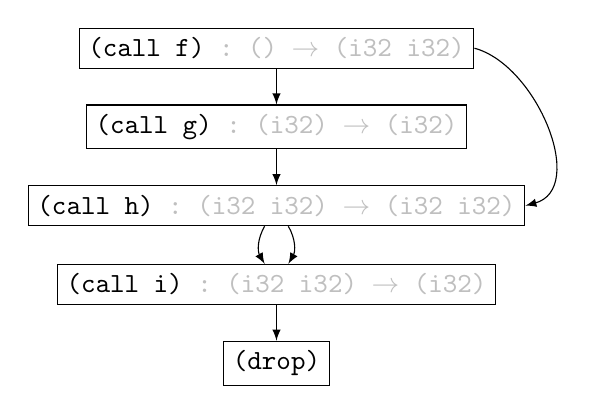
\begin{tikzpicture}
    \node[draw] (f) at (0, 0) {\texttt{(call f)\color{lightgray}~:~() $\to$ (i32 i32)}};
    \node[draw] (g) at (0, -1) {\texttt{(call g)\color{lightgray}~:~(i32) $\to$ (i32)}};
    \node[draw] (h) at (0, -2) {\texttt{(call h)\color{lightgray}~:~(i32 i32) $\to$ (i32 i32)}};
    \node[draw] (i) at (0, -3) {\texttt{(call i)\color{lightgray}~:~(i32 i32) $\to$ (i32)}};
    \node[draw] (d) at (0, -4) {\texttt{(drop)}};

    \draw[->,>=latex] (f) to (g);
    \draw[->,>=latex] (f.east) to[in=15, out=-15] (h.east);
    \draw[->,>=latex] (g) to (h);
    \draw[->,>=latex] (h) to[bend right] (i);
    \draw[->,>=latex] (h) to[bend left] (i);
    \draw[->,>=latex] (i) to (d);
  \end{tikzpicture}
  \caption{Non classical data flow with multiple return values}\label{data-flow}
\end{figure}

\textsf{Watib}'s IR is closer to modern Wasm. We represent the instructions in a
linear way. It allows to output code that use block parameters without
additional burden for instance. We hope that will enable different optimisations
and a better treatment of code written using WebAssembly's new features.

\section{Validation}\label{val}
We start by giving an overview of WebAssembly's type system, and then describe
our implementation of type checker for it. The abstract syntax of types is
presented in Section~2 of the specification and the rules of typing and
subtyping are presented in Section~3. We focus on the subtyping relation and the
typing of instructions as the rest of the validation is straightforward
(checking some names don't appear twice, global variables' initial values are
constant, etc.).
\subsection{WebAssembly's type system}
We present the types used in WebAssembly and some declarative rules for
subtyping and typing of instructions.
\subsubsection{Contexts}
We state all the following rules in an implicit \emph{context}. We will refer to
it as $C$ in the formal rules. Contexts are records; the only relevant field in
the following is \textsf{types} which maps type indices to \emph{defined types}
as defined in~\ref{deft}.

\subsubsection{Value Types}
WebAssembly is statically typed. Its main types are \emph{value types}, which
will be noted $t, t_1, t_2, \ldots$. They are the types of values on the stack.
They can be \emph{numeric types} (\textsf{i32}, \textsf{f64}, etc.),
\emph{vector types} (\textsf{v128}) or \emph{reference types}. The latter
represents pointers to functions, pointers to objects allocated on the heap
(structures or arrays, called \emph{aggregates}) or unboxed integers (using
tagged pointers). Each reference type is either nullable ($\refnullt ht$) or not
($\reft ht$), where $ht$ is a \emph{heap type}. Such a type is either an
\emph{abstract heap type} which we do not detail here or a type index referring
to one of the three following possibilities.
\begin{itemize}
  \item \emph{Function types} are written
$\funt{t_1}^*\to{t_2}^*$ (recall a function can have multiple outputs).
  \item \emph{Array types} are written $\arrt mut\ t$, where $mut$ denotes the
mutability of the array. It is \textsf{var} for a mutable array and
$\textsf{const}$ otherwise.
\item \emph{Structure types} are written $\strt
  {(mut\ t)}^*$. All these types are ordered by a subtyping relation we detail
in~\ref{func-aggr}.
\end{itemize}

\subsubsection{Instruction types}
Inference rules are given in the specification to give \emph{instruction types}
to instructions. These types indicate which values on the stack an instruction
pops, which values it pushes and which local variables it sets\footnote{to
forbid, at the type level, using a variable not initialised yet}. We omit this
last information in our presentation to stay simple. We write \emph{instruction
types} as function types: ${t_1}^*\to{t_2}^*$ for an instruction that pops
${t_1}^*$ and pushes ${t_2}^*$. We have the classical rule of subtyping for
functions~\cite{cardelli1988semantics} on these types: an instruction can accept
smaller types as inputs and produce bigger types as outputs. An additional
subtyping rule is added to reflect the stack-based semantics of Wasm : we can
add arbitrary value types before the input and output types as long as we add
the same on both. These rules are formalised in Figure~\ref{subinstr}.

A sequence of instructions can then be typed by the composition of types derived
for each of its instruction. For instance, the sequence \texttt{(i32.const~0)
  (i32.const~0) i32.add} can be typed $()\to(\text{\textsf{i32}})$, by giving
the type $(\text{\textsf{i32}})\to(\text{\textsf{i32}}\ \text{\textsf{i32}})$ to
the second \textsf{i32.const} --- which shows the need for the second subtyping
rule.

\begin{figure}[h]
  \begin{mathpar}
    \inferrule{{\left(C\vdash t_1\leq t_1\right)}^*\\
      {\left(C\vdash t_2\leq t_2\right)}^*}
              {C\vdash {t_1}^*\to{t_2}^* \leq {t'_1}^*\to{t'_2}^*}\hspace{1in}
    \inferrule{\\}{C\vdash {t_1}^*\to{t_2}^* \leq t^*{t_1}^*\to t^*{t_2}^*}
  \end{mathpar}
  \caption{Subtyping rules for instruction types}\label{subinstr}
\end{figure}

\subsubsection{Function and aggregate types}\label{func-aggr}
We now give details on the definitions and subtyping of \emph{function types}
and \emph{aggregate types}. As shown in Figure~\ref{tdef}, Wasm allows the
definition of mutually recursive types. Moreover, it supports \emph{declared and
mutually iso-recursive subtyping}.

\begin{figure}[h]
  \begin{lstlisting}
(rec
  (type $a (array (ref $b)))
  (type $b (struct (field (ref null $c))))
  (type $c (func (param (ref $a)) (result (ref $c)))))
  \end{lstlisting}
  \caption{Some type definitions}\label{tdef}
\end{figure}

Function types are endowed with the same first rule described for instruction
types (the contravariant/covariant one). An array type $\arrt mut\ t$ is a
subtype of $\arrt mut'\ t'$ if $mut\ t\leq mut'\ t'$. It means that the
mutabilities are the same and that $t$ is a subtype of $t'$. When both types are
mutable we also require that $t'$ is a subtype of $t$, i.e. that both types are
equivalent. A structure type $\strt {(mut_i\ t_i)}_{i=1}^n {(mut\ t)}^*$ is a
subtype of $\strt {(mut'_i\ t'_i)}_{i=1}^n$, if $mut_i\ t_i\leq mut'_i\ t'_i$ for
all $1\leq i\leq n$.

\subsubsection{Declared subtyping}
Wasm's subtyping is \emph{declared} as the subtyping relations between the
defined types have to be specified as part of the type definition to be used.
Their validity can be checked with the type definition's validation. For
example, the definition of \texttt{\$pair} in Figure~\ref{ex} states that it is
a subtype of \texttt{\$pair-nil}. If the \texttt{(sub \$pair-nil \dots)} part
wasn't in the definition, the function's code would be invalid, as it relies on
this subtyping relation for the type tests and the casts.

\subsubsection{Mutually iso-recursive subtyping}\label{deft}
We now give the intuition behind \emph{mutually iso-recursive
subtyping}~---~see~\cite{rossberg2023mutually} for a full discussion. It is a
way to support subtyping in presence of mutually recursive type definitions,
while avoiding size blowups. When checking a block of mutually recursive type
definitions, we build an internal representation where indices referring to
types of the block have been replaced by special indices of the form $\rect i$
where $i$ is the position of the corresponding index in the block. The concrete
definitions of the types are then replaced by \emph{defined types} consisting of
the block of type definitions and an index. For instance, the block of
Figure~\ref{tdef} will be translated to the following internal representation:
\begin{align*}
\rect\ (& (\arrt \cstt\reft \rect 1)\\
&(\strt\ (\cstt \refnullt \rect 2))\\
&(\funt\ (\reft \rect 0)\to (\reft \rect 2))).
\end{align*}
Each type definition is then replaced with a reference to this block and an
index (0 for \textsf{\$a}, 1 for \textsf{\$b}, etc.).

Once we have this representation, a defined type $t$ will be a subtype of
another defined type $t'$ if they are equal or if $t$ is declared as a subtype
of a subtype of $t'$.

\subsubsection{Unrolling}
Defined types only give a block of definitions and an index. To retrieve the
corresponding concrete type, one uses \emph{unrolling}. It consists of replacing
a defined type of the form $(\rect st^*).i$ by the $i^{\text{th}}$ type of $st$
where the indices of the form $\rect j$ have been replaced by $(\rect st^*).j$.

\subsection{A type checker for WebAssembly}
\subsubsection{The problem of transitivity}
The typing rules given by the third section of the specification are purely
declarative. They give more than one type to many instructions and rely on the
transitivity rule of subtyping, which can't be implemented as is. If we want to
check that $t_1 \leq t_2$ in presence of transitivity, we need to choose a third
type to compare it to $t_1$ and $t_2$, which complicates subtyping. We, thus,
needed to adapt them to implement a type checker.

\subsubsection{Our solution}
Our type-checker is similar to the one shipped with the specification. For the
subtyping of \emph{value types}, we rewrote the rules to have equivalent ones
without the transitivity rules\footnote{they are implemented by the function
\texttt{<ht=} of the \texttt{Type/match.scm} and reproduced in
Appendix~\ref{subtyping}} and for \emph{instruction types}, we rely on a stack
and most general types, as explained in the next paragraph.

To check a sequence of instructions we maintain an internal state recording the
types of the elements present on the stack and then check instruction in order,
instead of analysing each instruction individually and checking that the types
compose well.

\subsubsection{Most-general instruction types}
Most instructions have a most general type (i.e.\ a type subtype of all the
other types we can type the instruction with) or are not exited (like
unconditional branches). The typing rules for the latter are $i:{t_1}^*t^*\to
{t_2}^*$ for all $t_1$ and $t_2$. We represent it as ${t_1}^*t^*\to {t_2}^*$,
where \textsf{poly} is a special symbol indicating that the stack can be
whatever we need it to be~---~it can be thought as a type variable, on which we
do not perform explicit unification. When we refer to the type one of those
instruction, we mean its most general type or the type with the \textsf{poly}
symbol, these types are contained in the file \texttt{Val/instruction-types.sch}.
The instructions that do not fall in either category (for instance,
\textsf{ref.as\_non\_null} has type $\refnullt ht\to \reft ht$ for all heap type
$ht$) are treated in a separate function, they peek on the stack to compute
their output type, avoiding the use of type variables.

\subsubsection{The algorithm}
We describe how one instruction $i$ modifies the state of this stack. Either the
instruction is treated in an ad-hoc way (function \texttt{adhoc-instr}), or we
apply the following procedure (function \texttt{valid-instr}):

\begin{itemize}
\item Let ${t_n\ldots t_1}^*\to{t'}^*$ be the type of $i$.
\item Check that the $i^{\text{th}}$ type on the stack is a subtype of $t_i$ and
  pop it, for $i$ from $1$ to $n$. If the stack is equal to \textsf{(poly)}, we
  consider that for all $i$, the $i^{\text{th}}$ type on the stack is
  $\bot$, making the previous test successful.
\item If ${t'}^*$ is equal to \textsf{(poly)}, replace the stack by
  \textsf{(poly)}, otherwise push the return types on top of the stack.
\end{itemize}

\subsubsection{Type checking blocks}
When checking the types of blocks we set the parameter types as initial state of
the stack and compare the final the state of the stack with the expected type.
For that final check, we pop types from the stack and make sure that they are
subtype of the expected ones. We then check that the resulting stack is empty or
equal to \textsf{(poly)}.

\section{Optimisation}\label{opt}
\textsf{Watib} performs several optimisation passes. They all take care to
maintain typing information. As we show it later, some code is unnecessary
execution-wise but needs to be kept to maintain well-typedness.

\subsection{Generic optimisations}
We start by reviewing optimisations which benefit the others, by giving more
precise information or removing generated useless code. They are generic, in the
sense that they are applied in most optimising
compilers~\cite{muchnick1997advanced}.

\subsubsection{Copy Propagation}
When a variable $x$ is assigned the value of another variable $y$, we replace
references to $x$ with references to $y$, until the next assignment to $x$ or
$y$. We were inspired by~\cite[Section~12.5]{muchnick1997advanced} approach to
local copy propagation.

We traverse a sequence of instruction while maintaining a table which indicates
if a variable has been assigned to another one and each enclosing label is
associated to a list of such tables. We then apply the following procedure when
encountering an instruction $i$:
\begin{description}
  \item[assignment] When $x$ is assigned a variable's $y$ value, the table is
    updated with $x$ pointing to $y$. Otherwise all the assignments concerning
    $x$ are removed from the table.
  \item[access] When accessing a variable that is bound to another one in the
    table, the instruction is modified to access the latter.
  \item[branch] When branching to a label $l$, the current table is appended to
    the list associated to $l$.
  \item[block] When entering a block, an empty list is associated with its
    label. The table after the block corresponds to the upper-bound of all the
    tables in the label's list and the table at the end of the block. The
    upper-bound of list of tables assigns $y$ to the $x$ if all tables do and
    gives no information on $x$ otherwise.
  \item[loop] When entering a loop, the table is reset to remove all the
    assignments as we may jump to the beginning of the loop from later in the
    block\footnote{this is suboptimal for global copy propagation, but it is
    sufficient for the code we get and this optimisation could be replaced by
    Static Basic Block Versioning~\cite{melanccon2024static} which we are trying
    to adapt to Wasm}.
  \item[try] When protecting a block with some \textsf{catch} clauses, the table
    indicating no assignment is appended to all the labels these clauses can
    jump to. Once again this is coarse.
\end{description}
\subsubsection{Pure Drops Elimination}
We eliminate \textsf{drop} instructions and
their argument when it has no side effect. We try to remove as extra
computation as possible by inserting as much \textsf{drop} as needed.

\subsubsection{Constant Folding}
We replace some expressions that can be evaluated at compile time by their
value. We also also remove conditional branching when the condition is constant.

\subsubsection{Unreachable Code Elimination}
We eliminate some instructions that are known to never execute (after a
\textsf{return} for instance). However, some dead code may be needed for
validation, even though it can't be executed. For instance, removing the
\textsf{unreachable} instruction at the end of the function of Figure~\ref{ex}
makes it ill-typed. The \textsf{if} instruction puts nothing on the stack while
the function expects an \textsf{i32} on top of the stack as it is its declared
return type. An \textsf{unreachable} instruction is inserted instead of the
unreachable code, when it isn't preceded by an instruction of polymorphic return
type such as a \textsf{return}.

\subsubsection{Peephole optimisation}
We recognise small patterns in Wasm code and replace them with equivalent code
that is smaller or faster. For instance a sequence of \textsf{local.set} and
\textsf{local.get} with the same variable can be replaced by a
\textsf{local.tee} which assigns to a variable the value on top of the stack
without popping it.

%% \subsubsection{Type propagation}
%% This one is not an optimisation \emph{per se}. It only refines type annotations
%% of variables in the IR. When a variable is assigned a value, the type of this
%% value (which may be a strict subtype of the variable's declared type) is set as
%% the actual output type of each variable access, until it is modified.

\subsection{Wasm specific optimisations}
We now review more Wasm-specific optimisations and detail in which way they use
the previous ones.
\subsubsection{Cast Elimination}
We eliminate redundant casts and replace type tests by constants if their result
can be determined. Such casts and tests could be introduced by copy-propagation
as when we may replace a variable with another one of a smaller type or by the
next optimisation. To stay conservative about side-effects eliminated tests are
replaced by a \textsf{drop} and the result of the test, which is a constant.
Pure Drop Elimination will remove some useless computation. Constant folding
will propagate the result of the test.

To check for type tests to eliminate, we compare the argument's actual type
(which may be smaller than its static type) against the type it is tested for.
For casts, we only check against the static type as the cast can be necessary to
maintain well-typedness.

\subsubsection{Type-Dependent Control Flow Rewriting}
A common pattern in the Wasm code generated during the compilation of
dynamically typed programming languages, such as Bigloo, is a branching on a
type test followed by the use of casts in the branch where the test is
successful, like in Figure~\ref{ex}. If Wasm wasn't statically typed, these
casts could be removed by an optimising compiler that would determine that they
are redundant.

To avoid useless type tests, we introduce $\broncast l\ rt_1\ rt_2$ where $l$ is
a label expecting a value of type $rt_2$ as parameter and $rt_1\geq rt_2$ are
reference types. It combines branching and casting. A call to this instruction
with a value of type $rt_1$ on top of the stack checks it against the type
$rt_2$. If it's of type $rt_2$ then it branches to label $l$ with the value on
top of the stack cast to $rt_2$ as a parameter, otherwise the execution
continues with no modification to the stack.

We have an optimisation pass replacing \textsf{if} instructions which branch on
a $(\reftest rt\ (\localget x))$ by calls to \textsf{br\_on\_cast}. We add a
local variable $y$ of type $rt$ and create a new block labelled $l$ with a
parameter of type $rt$. The else branch follows the \textsf{br\_on\_cast} which
branches to $l$. The block labeled by $l$ puts its parameter in the local
variable $y$, assigns the value of $y$ to $x$ and contains the then branch. This
last assignment will allow Copy Propagation to replace $x$ by $y$ when
appropriate. Cast Elimination then removes useless tests. This whole code in
contained in a block which the else branch goes to at the end. The
transformation is showcased in Figure~\ref{br}.

\begin{figure}[h]
  \centering
  \begin{tabular}{c c c}
    \begin{minipage}{\widthof{\texttt{(if (ref.test (ref \$pair)}}}
\begin{verbatim}
(if (ref.test (ref $pair)
      (local.get $x))
  (then B1)
  (else B2))
\end{verbatim}
\end{minipage}
    &
    $\rightarrow$
    &
\begin{minipage}{\widthof{\texttt{....(br\_on\_cast \$then (ref \$pair-nil)}}}
\begin{verbatim}
(local $y (ref $pair))
(block $end
  (block $then (result (ref $pair))
    (br_on_cast $then (ref $pair-nil)
                      (ref $pair)
      (local.get $l))
    (drop)
    B2
    (br $end))
  (local.tee $y)
  (local.set $x)
  B1)
\end{verbatim}
\end{minipage}
  \end{tabular}
  \caption{General form of type-dependent control flow rewriting}\label{br}
\end{figure}

While the code after the transformation is bigger, some instructions \texttt{(br
  \$end)} can be removed on real examples.

%% \subsection{Control-Flow Graph transformation}
%% \subsubsection{Control-Flow Graphs}\label{cfg}
%% Many optimisations and code transformations are expressed well on
%% \emph{Control-Flow Graph} (CFG). It is a graph whose nodes are \emph{basic
%% blocks} (sequences of instructions that do not affect the control flow, here
%% Wasm instructions) and arcs represent potential jumps. To reflect the typing
%% discipline of Wasm, we consider CFGs whose basic blocks have instruction types.

%% We are working to adapt Static Basic Block Versioning or SBBV~\cite{melanccon2024static}
%% (which requires CFGs) to WebAssembly. It could subsume many of our passes and
%% remove type tests.
%% \subsubsection{Construction of a control-flow graph}
%% Constructing a CFG from a Wasm program is straightforward except for exceptions
%% which we don't support yet. One only needs to follow the programs control flow.
%% While instruction sequences are explored, a current state of the types on the
%% stack is recorded and used to put type annotation on the basic blocks.
%% \subsubsection{Reconstruction of Wasm}
%% As we don't have a general goto instruction, some work has to be done to recover
%% a valid Wasm program from a CFG. To do it, we implement the algorithm described
%% in~\cite{ramsey2022beyond}. This algorithm relies on the \emph{dominance tree}
%% of the CFG, which we compute using the algorithm of~\cite{cooper2001simple}.

%% Ramsey's algorithm works on \emph{reducible} CFGs. Intuitively, a CFG is
%% reducible when each loop has a single entry point\footnote{this is actually a
%% formal definition of reducibility if we define loops and their entry points}.
%% WebAssembly's structured control flow only produce such CFGs. But the SBBV we
%% work on can modify the CFG of a program with no guaranty on reducibility, at
%% least in its current formulation.

%% A irreducible CFG can be transformed in a reducible one using a technique
%% \emph{node splitting}~\cite[Appendix~A]{ramsey2022beyond}. It works by copying
%% some basic blocks until the resulting CFG is reducible. We plan on implementing
%% controlled node splitting as described in~\cite{janssen1997making} to obtain a
%% reducible CFG.
\section{Benchmarks}\label{bench}
\section{Conclusion}
We reviewed and motivated some of \textsf{watib}'s design choices and we
compared it to existing toolchains. We also detailed the type checking algorithm
and the optimisation passes.

\printbibliography
\newpage
\appendix
\section{Wasm-as' extensions to the specification}\label{wasmasex}
We try to list wasm-as' extensions to the spec, i.e. code modification made by
wasm-as silently that do not appear specification. To our knowledge, this
behaviours are not documented. The list is non-exhaustive. Feel free to contact
us if you find anything missing.
\subsection{\textsf{Unreachable} insertion}
Wasm-as tend to replace dead code code by \textsf{unreachable} and add
\textsf{unreachable} after blocks that don't exit. While semantically
preserving, this transformation can transform invalid code in valid code. For
instance, the following function is not well-typed according to the spec. But
wasm-as inserts an \textsf{unreachable} at the end, making it well-typed.
\begin{lstlisting}
(func (result i32)
  (if (i32.const 0)
    (then (return (i32.const 0)))
    (else (return (i32.const 0)))))
\end{lstlisting}

In the following piece of code, the \textsf{br} is not well-typed but wasm-as accepts
it:
\begin{lstlisting}
(func
  (result i32)
  (block $main (result i32)
    (i32.const 0)
    (if
      (then (return (i32.const 0)))
      (else (return (i32.const 0))))
    (br $main)))
\end{lstlisting}
\subsection{Automatic function reference declaration}
According to the specification, functions appearing in a \textsf{ref.func} have to
appear outside the function bodies (in a global or in an elem section). Wasm-as
puts all the undeclared function reference in an \textsf{elem declare func} section.

\subsection{Sign extension insertion for packed get}
According to the specification, when using \textsf{array.get} or
\textsf{struct.get} on a packed field (\textsf{i8} or \textsf{i16}), a sign
extension has to be specified. It means that either \textsf{.get\_u} or
\textsf{.get\_s} has to be used. Wasm-as allows \textsf{.get} instructions on
packed types, defaulting to unsigned.

\subsection{Replacement of block input values by locals}
Binaryen's README mentions that block input values are represented in the IR by
\textsf{pop} subexpressions for \textsf{catch} blocks and not supported for the
others. It is not mentionned that code using block input values will be replaced
by the use local variables. For instance, the following code:
\begin{lstlisting}
(i32.const 0)
(block (param i32)
  (drop))
\end{lstlisting}
is assembled to:
\begin{lstlisting}
(i32.const 0)
(local.set 0)
(local.get 0)
(drop)
\end{lstlisting}
\section{Matching rules for heap types}\label{subtyping}
\begin{mathpar}
  \inferrule{t_1 = t_2}{C\vdash t_1\leq t_2}\hfill
  \inferrule{\\}{C\vdash \bot\leq t}\hfill
  \inferrule{C\vdash C.\text{\textsf{types}}[x]\leq t}{C\vdash x \leq t}\hfill
  \inferrule{C\vdash t \leq C.\text{\textsf{types}}[x]}{C\vdash t \leq x}\\
  \inferrule{C\vdash t\leq\text{\textsf{any}}}
            {C\vdash\text{\textsf{none}}\leq t}\hfill
  \inferrule{C\vdash t\leq\text{\textsf{func}}}
            {C\vdash\text{\textsf{nofunc}}\leq t}\hfill
  \inferrule{C\vdash t\leq\text{\textsf{extern}}}
            {C\vdash\text{\textsf{noextern}}\leq t}\hfill
  \inferrule{C\vdash t\leq\text{\textsf{exn}}}
            {C\vdash\text{\textsf{noexn}}\leq t}\\
  \inferrule{C\vdash t\leq\text{\textsf{any}}}
            {C\vdash t\leq\text{\textsf{eq}}}\hfill
  \inferrule{\\}{C\vdash\text{\textsf{i31}}\leq\text{\textsf{eq}}}\hfill
  \inferrule{\\}{C\vdash\text{\textsf{struct}}\leq\text{\textsf{eq}}}\hfill
  \inferrule{\\}{C\vdash\text{\textsf{array}}\leq\text{\textsf{eq}}}\\
  \inferrule{\text{\textsf{unroll}} (deftype)= (symbol\ldots)}
            {C\vdash deftype\leq symbol}\hfill
\inferrule{\text{\textsf{unroll}} (deftype)= (symbol\ldots)\\ C\vdash symbol\leq\text{\textsf{eq}}}
            {C\vdash deftype\leq\text{\textsf{eq}}}
\end{mathpar}
\end{document}
